\newpage % Rozdziały zaczynamy od nowej strony.
\section{Eksperymenty}
\subsection{Zbiór  danych}
Dane są kluczową częścią głębokiego uczenia. Duży zbiór danych oznaczonych adnotacjami na poziomie pikseli jest potrzebny do wytrenowania wydajnego modelu segmentacji semantycznej. Typowe zestawy danych do segmentacji semantycznej to Cityscapes, PASCAL VOC i ADE20K. Podobnie w przypadku klasyfikacji sceny wymagany jest duży zbiór danych z odpowiednią informacją o etykiecie. Popularne zestawy danych do klasyfikacji scen obejmują  NYUv2, SUN RGB-D, Matterport3D i ScanNet.

Zbiór danych powinien ściśle odpowiadać założeniom postawionym w pracy. Zatem zbiór danych powinien zawierać kategorie scen, segmentacje obrazów 

Po prześledzeniu wielu zbiorów danych udało się sprostać powyższym wymaganiom, uzyskując dwa podobne zbiory danych - \texttt{NYUv2} oraz \texttt{SUN RGBD}. Ostatecznie wybrano \texttt{NYUv2} z uwagi, że zbiór ten został zawiera zdjecia
pomieszczeń, w które nie są posprzątane. Fakt ten uznano, za ważny, iż uważano, że będzie przekładał się na lepsze rezultaty w naturalnych warunkach. Co więcej \texttt{NYUv2} jest też chętniej cytowany niż \texttt{SUN RGBD} (rys. \ref{fig:sun-vs-nyu}).

\begin{figure}[ht!]
    \centering
    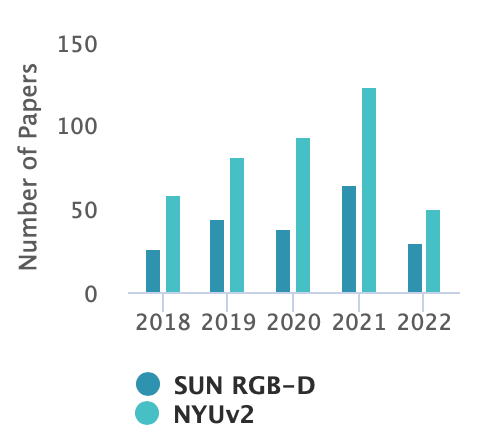
\includegraphics[width=0.5\textwidth]{img/stats-dataset.png}
    \caption[]{Szacowana liczba cytowań w latach 2018-2022 \href{https://paperswithcode.com/dataset/sun-rgb-d}{[paperswithcode.com]}}
    \label{fig:sun-vs-nyu}
\end{figure}

\subsection{Analiza zbioru danych}
Eksploracyjna analiza danych (ang. EDA) to proces eksploracji i zrozumienia cech zbioru danych przed zbudowaniem modelu. Omówione zostanie znaczenie EDA w głębokim uczeniu oraz możliwości wykorzystania do poprawy wydajności i interpretowalności modeli głębokiego uczenia.

\noindent
Jakość danych

Jednym z głównych powodów, dla których EDA jest ważne w wizji komputerowej, jest to, że może pomóc w identyfikacji problemów ze zbiorem danych, takich jak brakujące wartości, wartości odstające lub nieprawidłowe etykiety, które mogą wpłynąć na wydajność modelu wizji komputerowej. Przeprowadzając EDA, możemy uzyskać głębsze zrozumienie danych i zidentyfikować wszelkie problemy, które należy rozwiązać przed zbudowaniem modelu.

\noindent
Wstępne przetwarzanie danych

EDA może być również wykorzystana do określenia, które kroki przetwarzania wstępnego (ang. preprocessing), takie jak augmentacja, są niezbędne do poprawy wydajności modelu wizji komputerowej. Badając dane i rozumiejąc ich charakterystykę, jesteśmy w stanie lepiej dostosować różne techniki wstępnego przetwarzania danych.

\noindent
Identyfikacja tendencyjności

EDA może być również wykorzystana do identyfikacji potencjalnych błędów w zbiorze danych, takich jak skośne rozkłady klas, które mogą wpływać na wydajność modelu widzenia komputerowego i prowadzić do niesprawiedliwych prognoz. Przeprowadzając EDA, możemy zidentyfikować wszelkie uprzedzenia w danych i podjąć kroki w celu ich rozwiązania przed zbudowaniem modelu.

% Wnioski

% Podsumowując, prowadzenie EDA jest ważne w wizji komputerowej, ponieważ może pomóc poprawić wydajność modelu, zwiększyć jego interpretowalność i zapewnić, że model jest sprawiedliwy i bezstronny. EDA może być wykorzystana do identyfikacji problemów ze zbiorem danych, wyboru odpowiednich cech, wstępnego przetwarzania danych, zrozumienia zachowania modelu i zidentyfikowania potencjalnych stronniczości. Przeprowadzając EDA, możemy uzyskać głębsze zrozumienie danych oraz poprawić wydajność i interpretowalność modelu widzenia komputerowego.

EDA przeprowadzone na zbiorze NYUv2 dostarczyło wielu interesujących szczegółów. W zbiorze domyślnie znajduje się 795 przykładów trenujących oraz 654 przykładów testujących. Ze zbioru testowego wyodrębniono zbiór walidacyjny stanowiący 20\% zbioru testowego. Ponadto sprawdzono rozkład klas na przesztrzeni całego zbioru danych.
W przypadku zadania segmentacji semantycznej do dyspozycji był wybór 894, 40 lub 13 klas przedmiotów. Im rozróżnialność była większa tym większe okazywały się dysproporcje w rozkładzie. Histogramy dla 13 i 40 klas przedstawiono na rysunku \ref{fig:rozklad-segm}.
Podobna sytuacja miała miejsce dla zadania klasyfikacji z tą różnicą, iż scalania klas należało dokonać ręcznie. Taki krok był kluczowy, gdyż pierwotny rozkład był silnie zdominowany przez kilka klas.
Ostatecznie wybrano 13 klas dla klasyfikacji (rys. \ref{fig:7 klas dystrybucja}) oraz scalone 7 dla segmentacji (rys. \ref{fig:7 klas dystrybucja}).
\begin{figure}[ht!]
    \centering
    \begin{subfigure}[b]{0.49\textwidth}
        \centering
        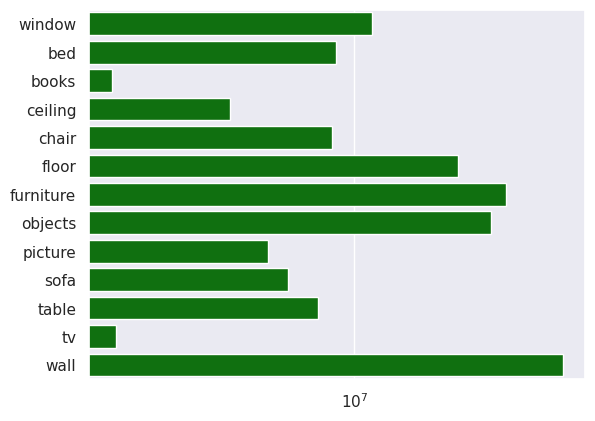
\includegraphics[width=\textwidth]{seg13.png}
        \caption{Rozkład dla 13 klas.}
        \label{fig:rozklad-13klas-seg}
    \end{subfigure}
    \hfill
    \begin{subfigure}[b]{0.49\textwidth}
        \centering
        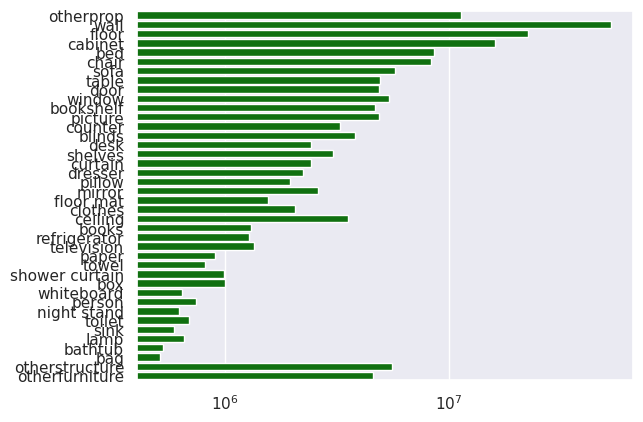
\includegraphics[width=\textwidth]{seg40.png}
        \caption{Rozkład dla 40 klas.}
        \label{fig:rozklad-40klas-seg}
    \end{subfigure}
    \caption[]{Porównanie rozkładu ilości pixeli dla zadania segmentacji semantycznej.}
    \label{fig:rozklad-segm}
\end{figure}
\begin{figure}
    \centering
    \begin{subfigure}[b]{0.49\textwidth}
        \centering
        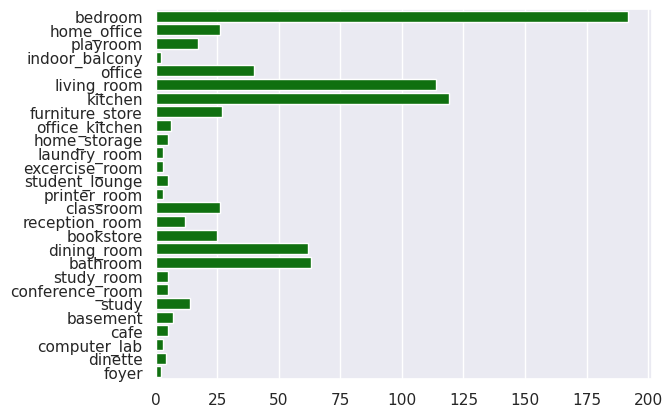
\includegraphics[width=\textwidth]{classification.png}
        \caption{Oryginalny rozkład klas.}
        \label{fig:27 klas dystrybucja}
    \end{subfigure}
    \hfill
    \begin{subfigure}[b]{0.49\textwidth}
        \centering
        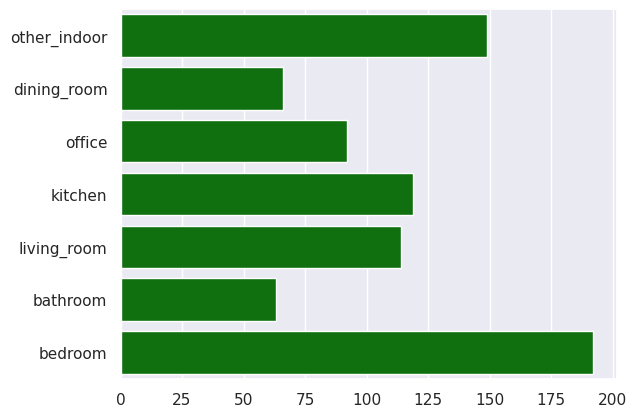
\includegraphics[width=\textwidth]{classification-merged.png}
        \caption{Rozkład klas po scaleniu.}
        \label{fig:7 klas dystrybucja}
    \end{subfigure}
    \caption[]{Porównanie rozkładu klas dla zadania klasyfikacji sceny.}
\end{figure}

% * wykorzystanie TU NICR
% * Wersje segmentacji: 13, 40 i 8xx klasowa
% * ile obrazków w jakich zbiorach.
% * wstawić przykładowe obrazki z datasetu
% * Konkatenacja dla klas dla klasyfikacji - dlaczego?
% * EDA - histogramy klas

\subsection{Opis eksperymentów}
\noindent
Przygotowanie danych

Obrazy RGB zostały poddane normalizacji ze średnią (0.485, 0.456, 0.406) oraz odchyleniem standardowym (0.229, 0.224, 0.225), która odpowiada parametrom rozkładu normlanego na zbiorze ImageNet. Baza ImageNet służyła do wytrenowania enkodera, a więc pierwszej części modelu.

Istnieje kilka różnych technik normalizacji, które mogą być stosowane w problemach z widzeniem komputerowym, takich jak normalizacja min-max i normalizacja rozkładem normalnym.  W pracy ,,Normalization Techniques in Training DNNs:
Methodology, Analysis and Application'' Lei et. al. \cite{huang2020normalization}, autorzy udowadjniają, że normalizacja stabilizuje i przyśpiesza trening oraz prawdopodobnie prowadzi do
do poprawy generalizacji. 

Normalizacja jest ważnym krokiem przetwarzania wstępnego w problemach widzenia komputerowego, ponieważ może pomóc w poprawieniu wydajności modelu. Normalizacja odnosi się do procesu skalowania danych wejściowych tak, aby miały w przybliżeniu średnią 0 i odchylenie standardowe 1. Pomaga to zapewnić, że dane wejściowe są w spójnym zakresie i mają podobny rozkład, co może poprawić model.
\noindent
Model

Jako  model użyto DeepLabv3, który rozszerzono o dodatkową głowę klasyfikacyjną. Umieszczono ją naturalnie zaraz za enkoderem, a przed dekoderem. Głowa klasyfikacyjna przedstawia się jako jako sieć w pełni połączona (FC) z dwiema warstwami.  

TO TRZEBA ZWIUZALIZOWAĆ!
\begin{addmargin}[6mm]{0mm}
    \begin{lstlisting}[
        language=Python,
        numbers=left,
        firstnumber=1,
        caption={Struktura głowy klasyfikacyjnej},
        aboveskip=0pt
    ]
    nn.AdaptiveAvgPool2d((1, 1)),
    nn.Flatten(),
    nn.BatchNorm1d(num_filters),
    nn.Dropout(p=0.25),
    nn.Linear(num_filters, out_features=256, bias=False),
    nn.ReLU(inplace=True),
    nn.BatchNorm1d(256),
    nn.Dropout(p=0.25),
    nn.Linear(in_features=256, out_features=scene_classes, bias=False),
    \end{lstlisting}
    \end{addmargin}

\noindent
Funkcja straty

W obu przypadkach jako funkcję straty wykorzystano ważoną entropię skrośną. Wagi odzwierciedłały odwrotność liczności w zbiorze. Dla klasyfikacji liczona była ilość klas, natomiast dla segmentacji ilość pixeli.

\noindent
Uczenie

sssssssss

\subsection{Wyniki}
W tym rozdziale zostaną przedstawione empiryczne wyniki badań nad wspólną segmentacją semantyczną i klasyfikacją sceny w środowiskach wewnętrznych. Badania mają na celu opracowanie i ocenę różnych znanych i aktualnych technik uczenia głębokich sieci neuronowych. Aby to osiągnąć, przeprowadzono serię eksperymentów na zbiorze na reprezentacyjnych zbiorach danych. Analiza dotyczyła zarówno miar jakości sensu stricto jak i miar wydajnośiowych proponowanych metod. Rozważono różne metryki oceny, takich jak ogólna dokładność, indeks Jaccarda  znany w literaturze jako intersection over union (IoU), miara F1 i wydajność obliczeniowa. Wyniki uzyskane w tym rozdziale zapewnią cenny wgląd w mocne strony i ograniczenia proponowanych metod. 

W pierwszej kolejności metody zostaną zbadane pod względem wymienionych wcześniej miar jakości w postaci ogólnej - niezagregowanej, osobno dla segmentacji oraz klasyfikacji. Omawiane metryki należy rozumieć jako średnia miara jakości na każdej z klas, a więc makrośrednie. Makrośrednie metryki są stosowane przy ocenie wydajności algorytmów dla zadań takich jak segmentacja semantyczna i klasyfikacja sceny, ponieważ zapewniają bardziej wszechstronną ocenę ogólnej jakości algorytmu. Metryki makrośrednie uwzględniają wydajność algorytmu na wszystkich klasach obiektów i regionów w obrębie sceny, a nie tylko koncentrują się na jakości na najbardziej powszechnych lub najłatwiejszych do sklasyfikowania klasach. W przypadku stosowania metryki makrośredniej jakość dla każdej klasy jest obliczana oddzielnie, a ogólna jakość jest obliczana jako średnia jakości poszczególnych klas. Stanowi to kontrast do metryki mikrośredniej, która oblicza ogólną jakość poprzez zsumowanie całkowitej liczby wyników  dla wszystkich klas.
Użycie makrośrednich metryk może być szczególnie ważne w scenariuszach, w których liczba instancji każdej klasy jest niezrównoważona lub gdy istnieje duża liczba klas. W takich przypadkach, mikrośrednie metryki mogą być mylące, ponieważ mogą być pod silnym wpływem najbardziej powszechnych klas, podczas gdy zaniedbują te mniej powszechne. Zatem makro analiza pokaże generalne rezultaty oraz otworzy dyskusję do dalszych, bardziej połgębionych badań na rozważanym problemem.

\vspace{0.5cm}
Rozpoczynając od segmentacji rozważamy 3 scenariusze testowe. Pierwszym z nich jest uczenie wyłącznie klasyfikacji rozumianej jako uczenie enkodera i sieci segmentacyjnej z pominięciem cześć klasyfikacyjnej. Pozwoli to odopwiedzieć na pytanie czy bardzie zaawansowane techniki uczenia polepszą, a może pogorszą działanie modelu. Drugim scenariuszem jest uczenie wielozadaniowe, gdzie cały model jest odmrożony, a błąd jest propagowany zarówno przez segmentację jak i klasyfikację. Ostanim eksperymentem jest sprawdzenie technik transferu wiedzy, a szczególne tak zwanego finetunowania. Model w pierwszym etapie uczy się przy zamrożnym enkoderze, dopiero na koniec jest odmrażany w celu dostrojenia wyników. 

\begin{figure}[ht!]
    \centering
    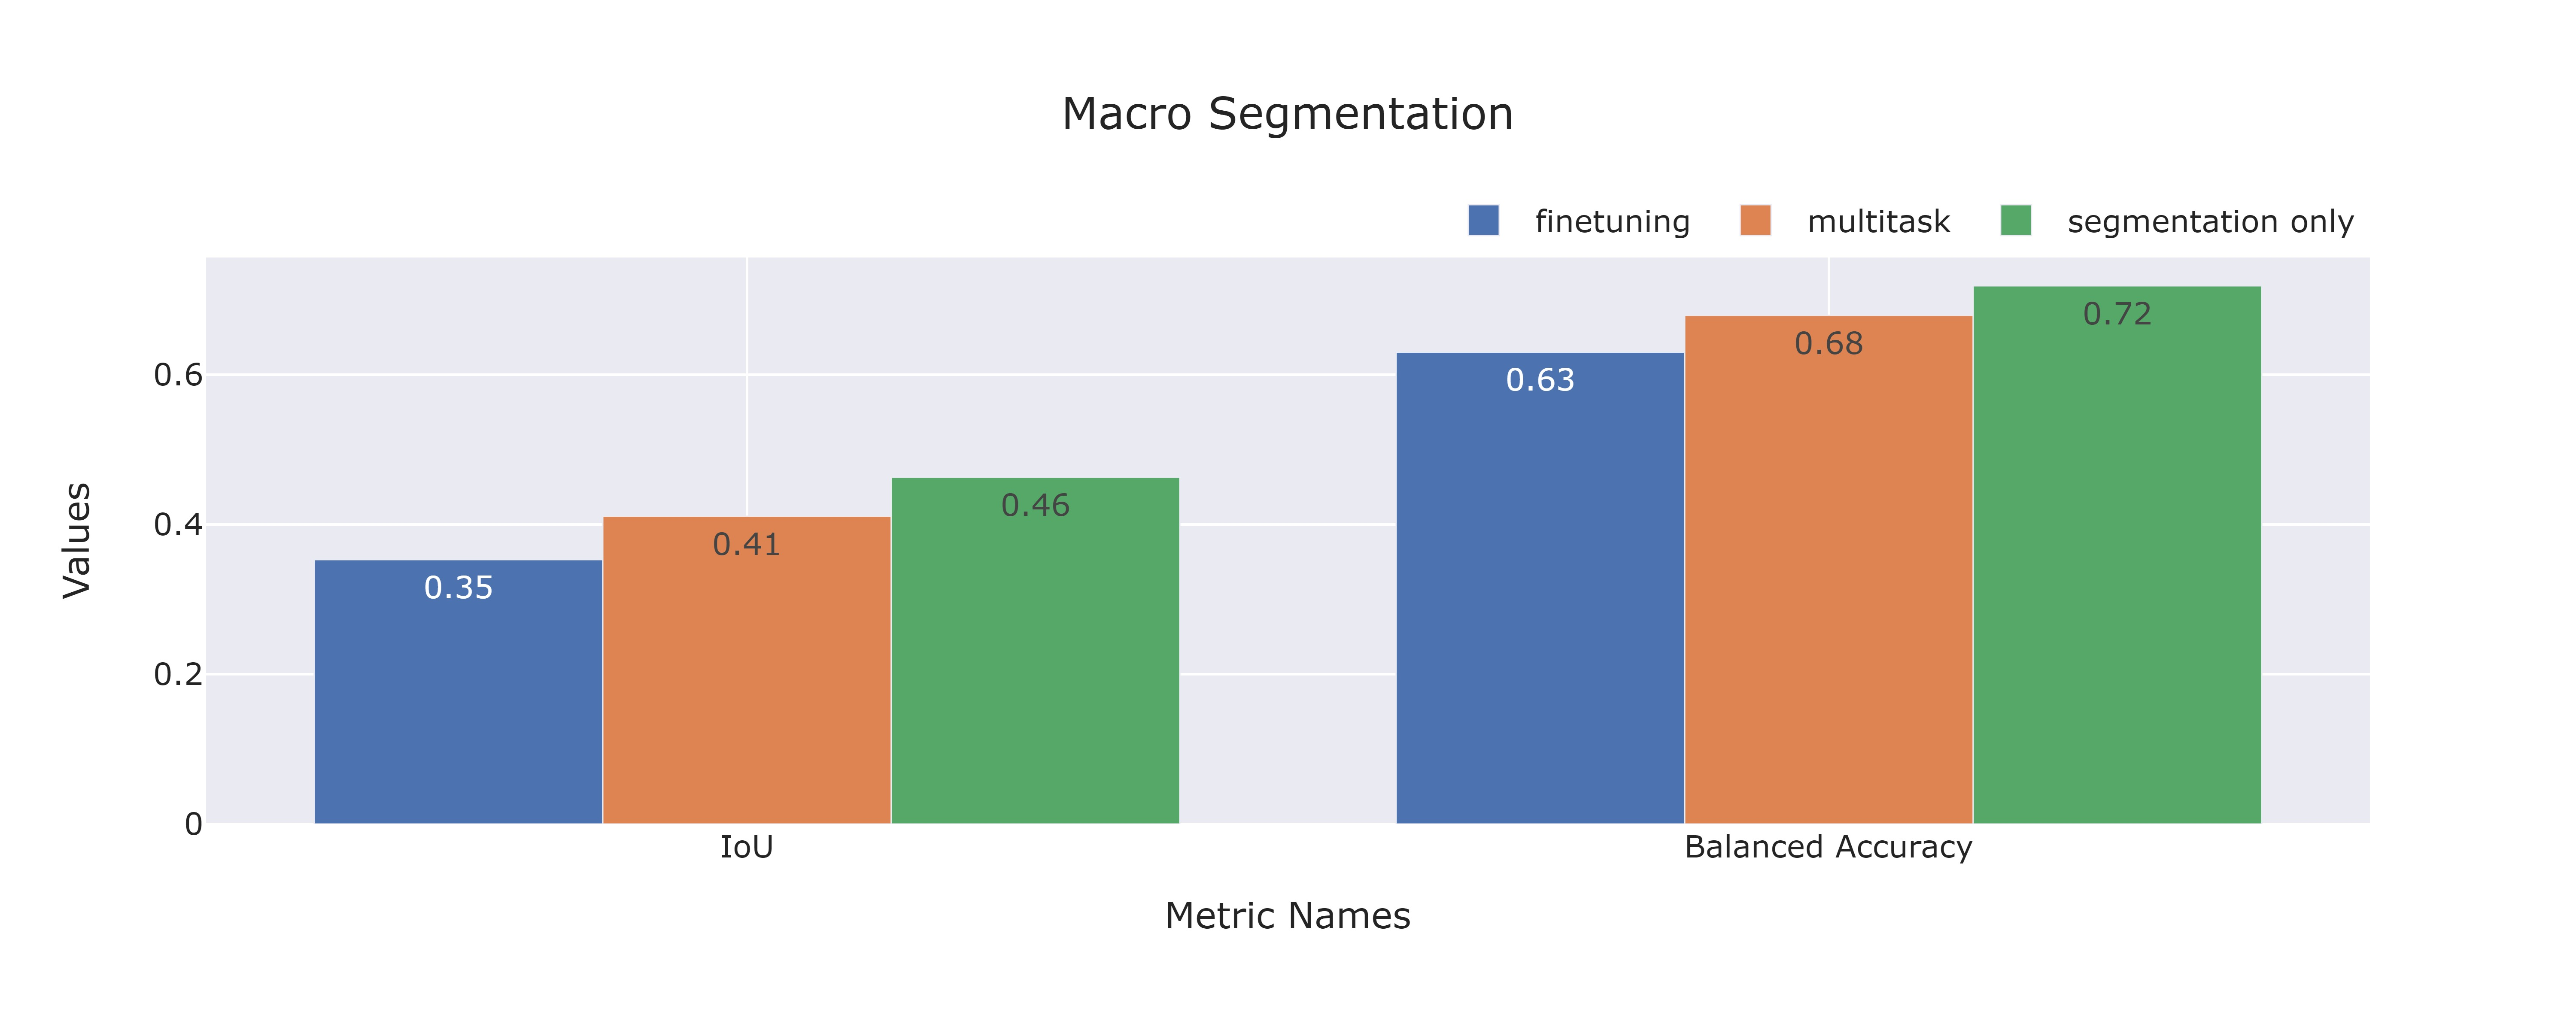
\includegraphics[width=\textwidth]{result_imgs_sorted/Macro-Segmentation.jpeg}
    \caption{Porównanie miar Iou oraz dokładnosci dla segmentacji sceny.}
    \label{fig:macro-segmentation}
\end{figure}

Analizując rysunek \ref{fig:macro-segmentation} nie trudno zauważyć, że najlepsze rezultaty otrzymano w dla uczenia wyłącznie segmentacji. Kolejnym wynikiem jest uczenie wielozadaniowe. Jako najsłabsze podejście okazuje się metoda finetunowania. Widać, że relacja jakości są zachowane dla każdej z metryk, a więc zarówno dla miary Iou jak i zbalansowanej dokładności (bAcc). Widać, że miara IoU wypada gorzej niż bAcc. Wyniką mogą sugerować, że trudno jest przeprowadzić transfer wiedzy z ImageNetu, gdyż finetunowanie wypada najsłabiej. Jest to naprawdopodobniej spowodowane zupełenie innym rozkładem klas dla wspomnianej bazie. Analiza sceny w przeciwieństwie do klasyfikacji najczęściej cechuje się długoogonowym rozkładem klas. Drugim instonym szczególem jest fakt, iż wagi dekodera i głowy segmentacyjnej są losowe. Uczenie wielozadaniowe zgodnie z zakłądanymi wynikami nie polepsza segmentacji, gdyż łączna przesztrzeń segmentacji i klasyfikacji jest niewątpliwie trudniejsza do optymalizacji. 

\vspace{0.5cm}
Przechodząc do klasyfikacji wyróżniamy 4 scenariusze testowe. Pierwzym jest uczenie wyłącznie klasyfikacji, analogicznie jak wyżej, a więc przy wyłączonej części segmentacyjenj. Kolejnymi są wspomiane wcześniej uczneie wielozadaniowe oraz finetuning. Nowym scenariuszem jest skorzystanie z wytrenowanej wcześniej wyłącznej segmentacji, a następnie wyłączenie wszystkiego poza siecią gęstą.
\begin{figure}[ht!]
    \centering
    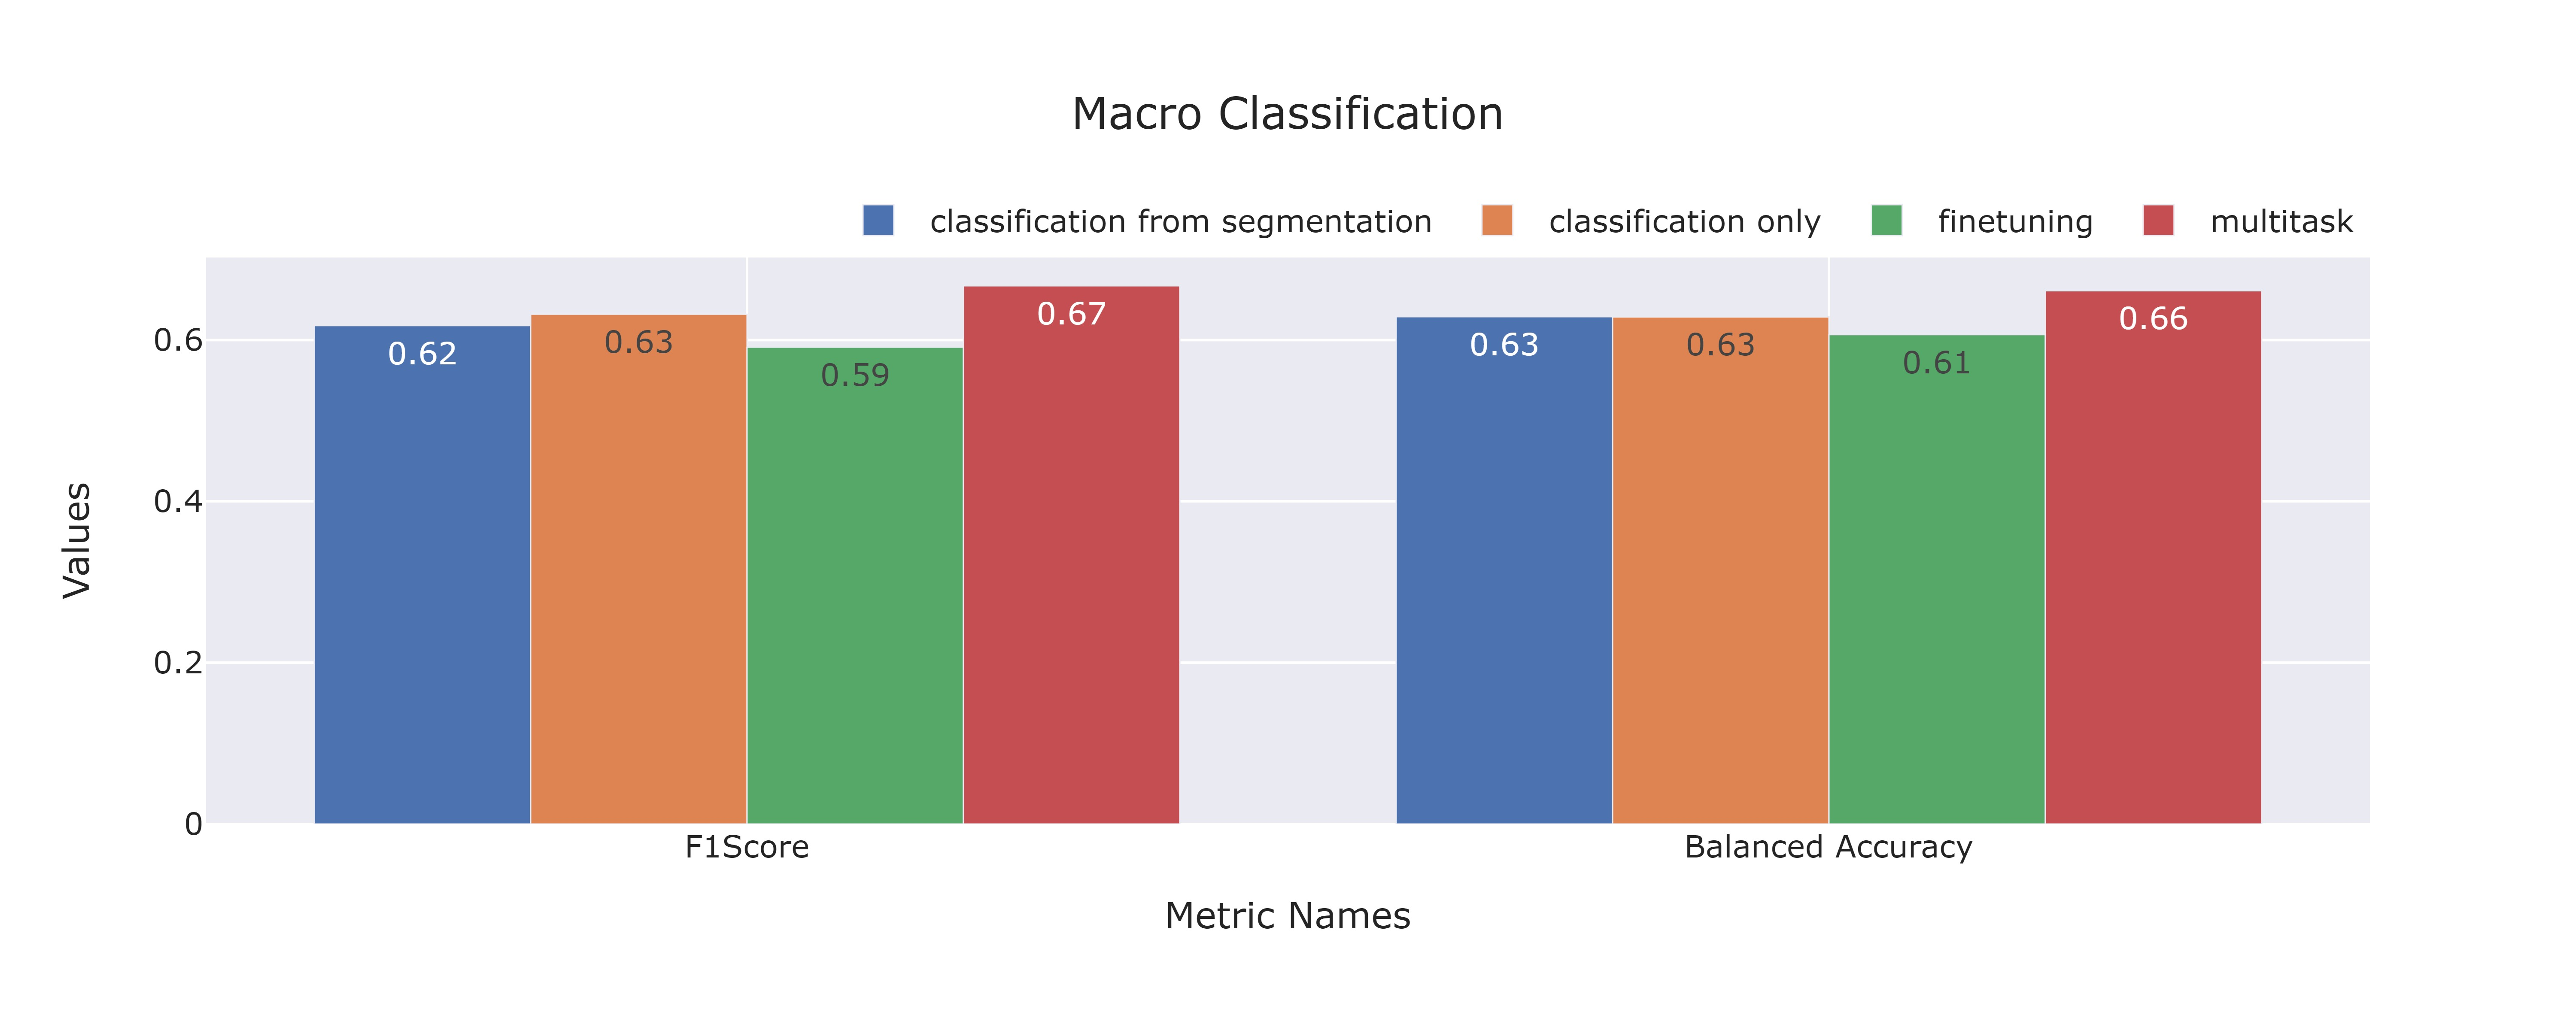
\includegraphics[width=\textwidth]{result_imgs_sorted/Macro-Classification.jpeg}
    \caption{Porównanie miar F1 oraz dokładnosci dla klasyfikacji sceny.}
    \label{fig:macro-classification}
\end{figure}

Rezultaty przedstawia rysunek \ref{fig:macro-classification}. Od razu da się zauważyć, że wyniki cechuje mniejsze odchylenie standardowe oraz,  analizujc łącznie miarę F1 oraz zbalansowaną dokładność, średnia. Fakt ten jest prawdopodbnie wynikiem znacznie mniejszej ilości parametrów uczących. Jako najlepszy rezultat uzyskuje uczenie wielozadaniowe. Ciekwym wydaje się fakt, że uczenie wyłącznie klasyfikacji jest słabsze w tym przypadku. Proadopodbnie poprzez uczenie wielozadaniowe enkoder wygenerował lepszą przestrzeń reprezentacji, co bezpośrednio wpływa na klasyfikację sceny.

\vspace{0.5cm}

Analizowanie jakości algorytmu dla każdej z klas osobno jest ważne, ponieważ pozwala na bardziej szczegółowe zrozumienie mocnych i słabych stron algorytmu. Rozważając ogólną jakość algorytmu przy użyciu metryki makrośredniej, nie jest od razu jasne, w których klasach algorytm radzi sobie dobrze, a z którymi ma problemy. Analizując jakość każdej klasy osobno, można zidentyfikować konkretne klasy, z którymi algorytm ma problemy i podjąć kroki w celu poprawy wydajności w tych klasach.


\vspace{0.5cm}
Rysunek \ref{fig:classification-accuracy} przedstawia dokładność dla każdej z klas dla zadania klasyfikacji sceny. Trudno jednozczanie określić która metod sprawdza się tutaj najlepiej. Uczenie wielozadaniowe wypada najlepiej dla klas: łazienka, pokój dzienny, salon, biuro. Uczenie wyłączenj klasyfikajcji jest najlpesze dla klas jadalnia oraz  kuchnia. W pozostałych przypadkach klasa inne pomiesczenia jest najlepiej wykrywana przez scenariusz finetunowania. Uczenie klasyfikacji z segmentacji nigdy nie osiąga najlpeszego wyniku.
\begin{figure}[ht!]
    \centering
    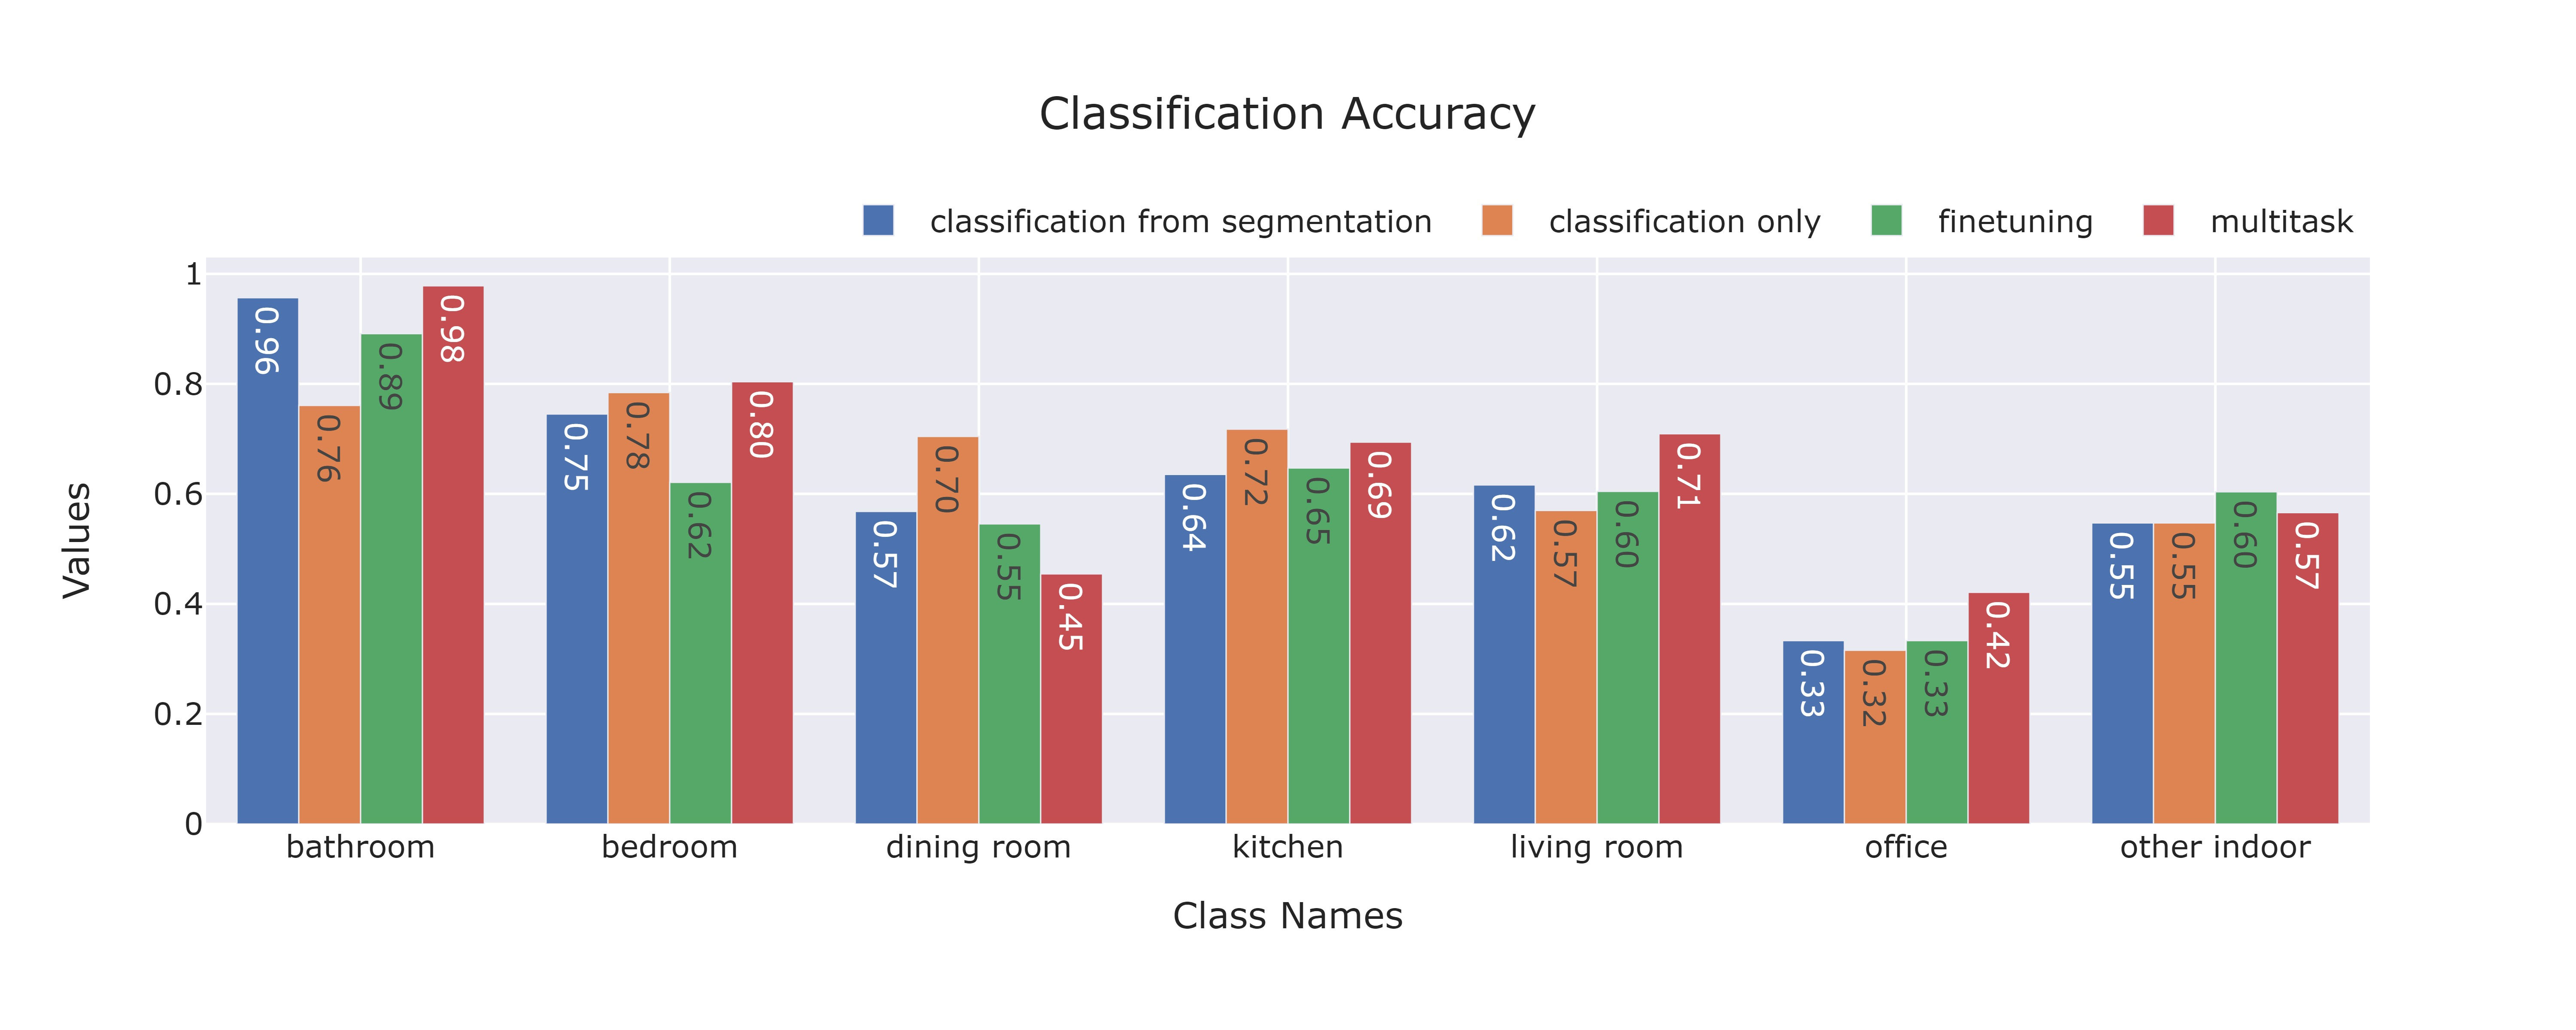
\includegraphics[width=\textwidth]{result_imgs_sorted/Classification-Accuracy.jpeg}
    \caption{Porównanie dokładności klasyfikacji sceny z rozróżniem konkretnych klas.}
    \label{fig:classification-accuracy}
\end{figure}
Biorąc pod uwagę miarę F1 (rys.\ref{fig:classification-f1}) rówznież nie jesteśmy w stanie wyróżnić faworyzowanej metody. W porówaniu z wcześniej analizowaną dokładnością widać, że uczenie wielozadaniowe utrzymuje w większości przypadku bardzo dobre rezultaty. Widać też, że wyniki w obrębie każdej z klas mało różnią się między sobą.
\begin{figure}[ht!]
    \centering
    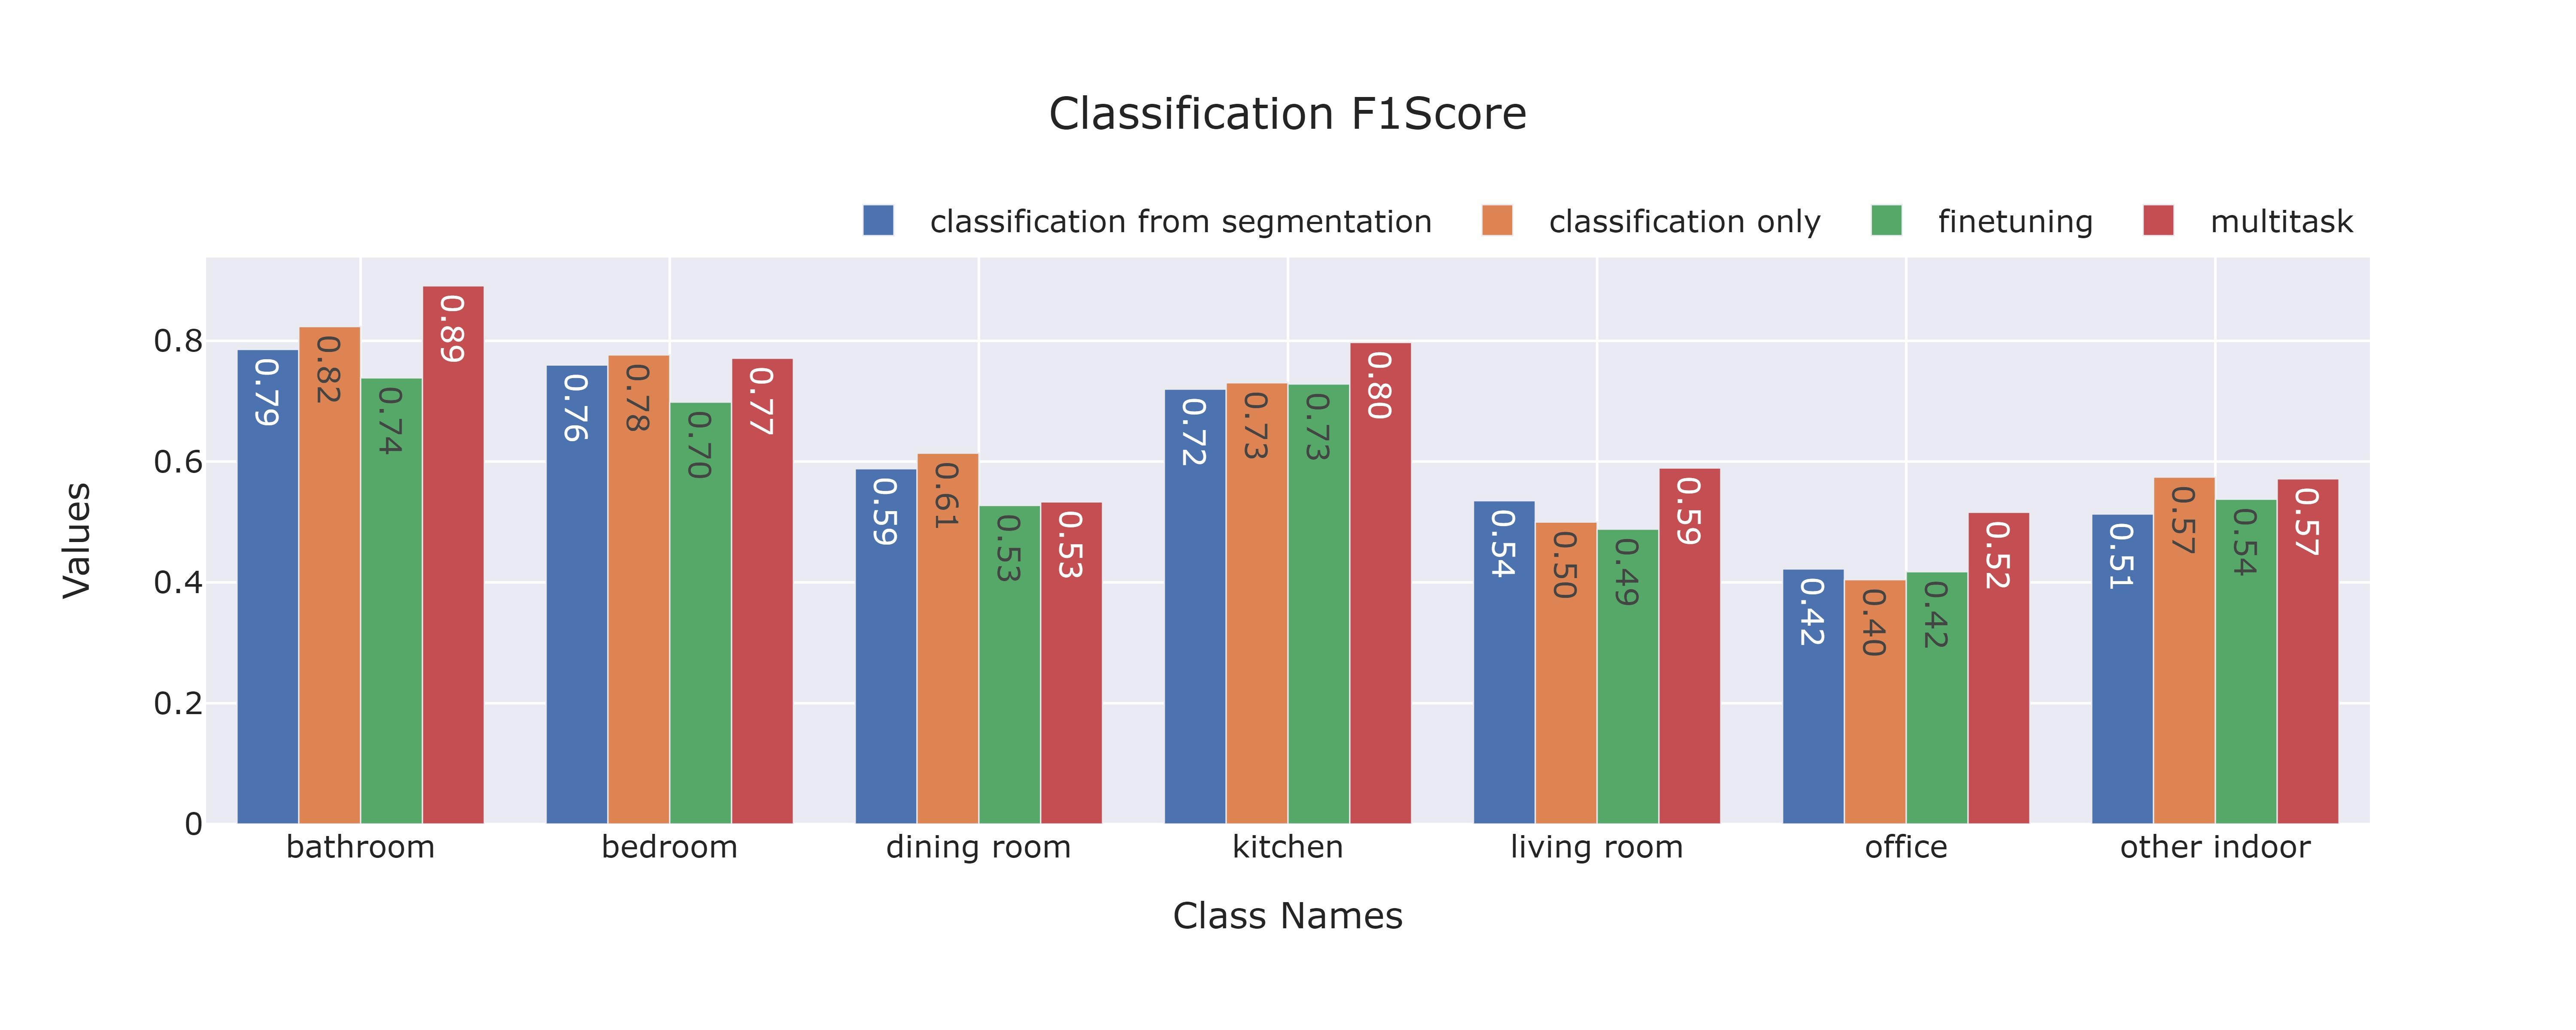
\includegraphics[width=\textwidth]{result_imgs_sorted/Classification-F1Score.jpeg}
    \caption{Porównanie miary F1 dla klasyfikacji sceny z rozróżniem konkretnych klas.}
    \label{fig:classification-f1}
\end{figure}

\vspace{0.5cm}

Anlizując rysunek \ref{fig:segmentation-acc} przestawiający dokładność w zadaniu segmentacji semantycznej, widać, że niektóre z zadań wypadają znacznie gorzej niż pozostałe. Sytuacja ta dotyczy klas meble, stóły, obiekty. Uczenie wyłącznie zegmentacji okazało się najlepsze dla klas łóżko, podłoga, meble, obiekty, obraz, tv, ściana oraz okno. Stanowi to ponad połowę wszytskich możliwych klas. Uczenie wielozadaniowe uzyskało najlepsze wyniki dla klas książki, sufit, sofa. Przypadek funetunowania nigdy nie osiągnął nalpeszego rezultatu.
\begin{figure}[ht!]
    \centering
    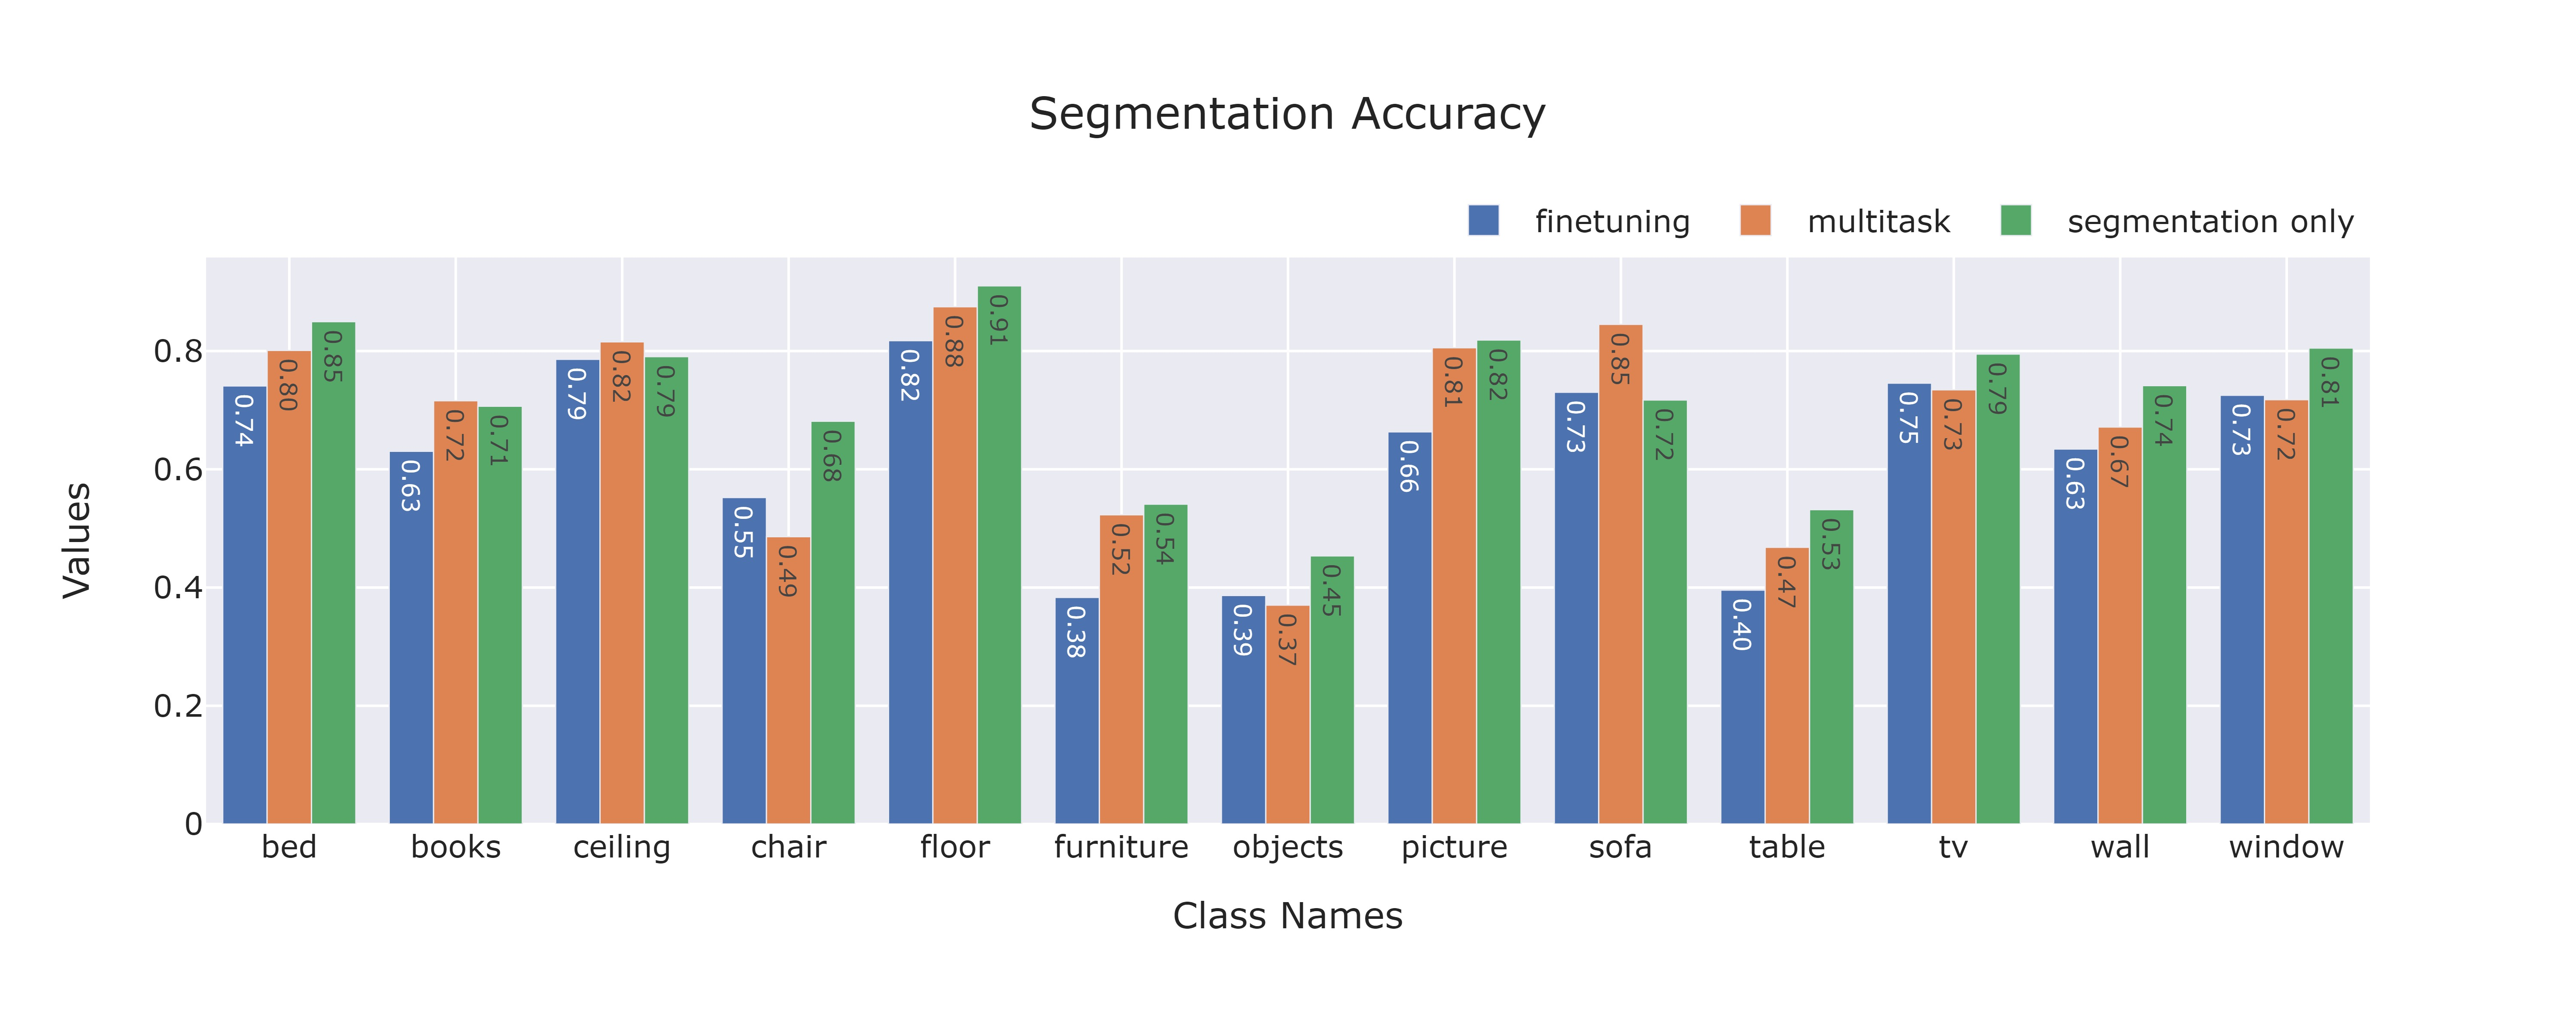
\includegraphics[width=\textwidth]{result_imgs_sorted/Segmentation-Accuracy.jpeg}
    \caption{Porównanie dokładności segmentacji z rozróżniem konkretnych klas.}
    \label{fig:segmentation-acc}
\end{figure}

Na rysunku \ref{fig:segmentation-iou} przestawiono IoU dla segmentacji semantycznej. Widać tutaj dużą dysproporcję miedzy klasami podłoga, ściana, a pozostałymi klasami. Jest to zrozumiałe, klasy te występują stosunkowo często na obrazie. Uczenie wyłącznie segmentacji uzyskuje najlepsze wyniki na wszytskich klasach z wyłaczeniem książek oraz telewizorów. W tych przypadkach najlepsze okazuje się uczenie wielozadaniowe
\begin{figure}[ht!]
    \centering
    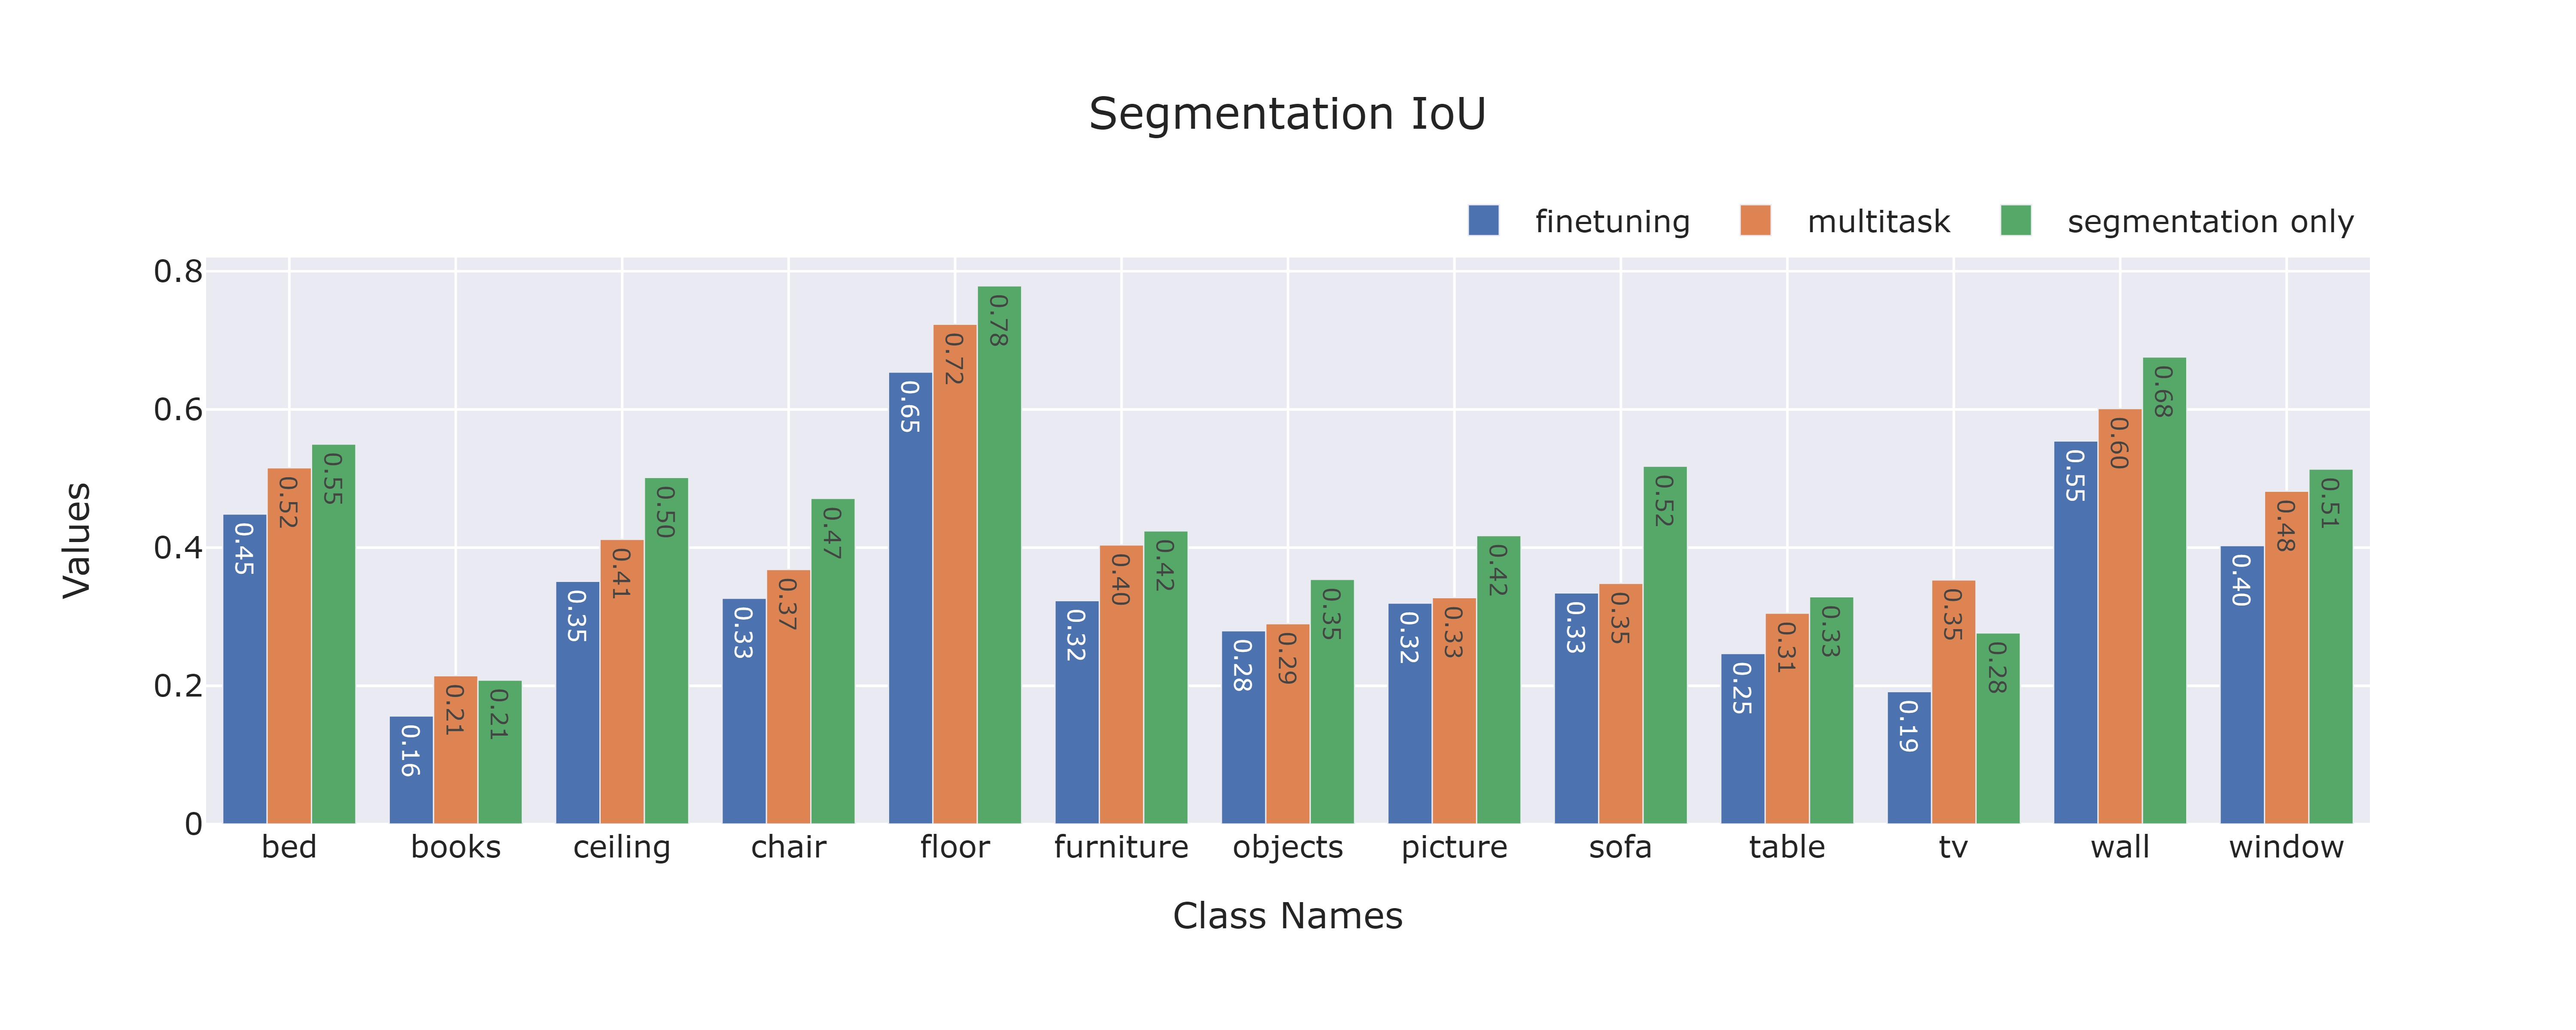
\includegraphics[width=\textwidth]{result_imgs_sorted/Segmentation-IoU.jpeg}
    \caption{Porównanie miary IoU segmentacji z rozróżniem konkretnych klas.}
    \label{fig:segmentation-iou}
    
\end{figure}
    % \begin{table}[]
    %     \centering
    %     \begin{tabular}{c|cc}
    %         zadanie/{[}\%{]} & Acc jednozadaniowe & Acc wielozadaniowe \\ \hline
    %         segmentacja      & 67.87               & 67.48  \footnotesize{\textbf{$-$0.39}}        \\
    %         klasyfikacja     & 65.50               & 67.45  \footnotesize{\textbf{+1.95}}        \\ \hline
    %     średnia          & 66.69               & 67.47  \footnotesize{\textbf{+0.78}}       
    % \end{tabular}
    % \caption{Porównanie dokładności dla uczenia jedno- i wielozadaniowe.}
    % \label{tab:acc-por}
    % \end{table}
    
    % \begin{figure}[ht!]
    %     \centering
    %     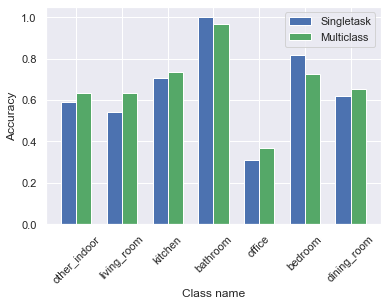
\includegraphics[width=0.75\textwidth]{scene_comp.png}
    %     \caption{Porównanie dokładności dla każdej z klas w zadaniu klasyfikacji pomieszczeń}
    %     \label{fig:scene_comp}
    % \end{figure}
    
    % \begin{figure}[ht!]
    %     \centering
    %     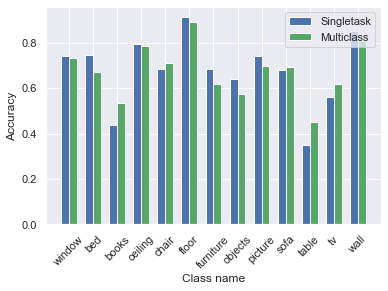
\includegraphics[width=0.75\textwidth]{seg_comp.png}
    %     \caption{Porównanie dokładności dla każdej z klas w zadaniu segmentacji semantycznej}
    %     \label{fig:seg_comp}
    % \end{figure}
    % Ucznie wielozadaniowe w rozważanym przypadku nieznacznie poprawia wyniki sieci (tab. \ref{tab:acc-por}). Dla zadania segmentacji semantycznej otrzymujemy spadek jakości o 0.39 punkta procentowego. Zadanie klasyfikacji poprawia się o 1.95 p.p. w porównaniu z uczeniem jednozadaniowym. Ostatecznie otrzymujemy zysk na poziomie 0.78 punkta procentego na średniej z zadań. Poprawa jest niewielka, jednak jest to dużu sukces biorąc pod uwagę, że mamy do dyspozycji 2 razy mniej parametrów niz w przypadku dwóch osobnych sieci. Przekłada się to bezpośrednio na czas inferencji, który w przypadku robotyki i systemów czasu rzeczywistego jest kluczowy.
    
    % Wartym zobaczenia jest fakt, iż uczenie wielozadaniowe poprawia wyniki dla klas które osiągają najsłabsze rezultaty w uczeniu jednozadaniowym. Poprawie ulega klasa office (rys. \ref{fig:scene_comp}) dla klasyfikacji oraz klasy books oraz table (rys. \ref{fig:seg_comp}) dla segmentacji semantycznej. Powodem jest prawdopodbnie mniejsze obciążenie (bias) modelu spowodowane faktem wzajemnej regularyzacji obu zadań w procesie uczenia. Innymi słowy, model ma mniejszą tendencję do przeuczenia.